\subsection{Найменша та найбільша нерухомі точки}
Для точкової міри $\mu$ на $[0, 1]$ визначимо відображення
$\min(\mu)$ та $\max(\mu)$, що ставлять у відповідність
цій мірі її найменший та найбільший атоми за формулами
\begin{gather}
    \min(\mu) = \sup \left\{x\in[0,1] :\mu([0, x]) = 0 \right\}, \\
    \max(\mu) = \inf \left\{x\in[0,1] :\mu([x, 1]) = 0 \right\},
\end{gather}
де для порожньої множини
покладаємо $\sup \varnothing = 0$ та $\inf \varnothing = 1$.
Якщо $\left\{x_1,\dots,x_k \right\}$ --- множина атомів $\mu$,
то  
$\min(\mu) = \min\left\{x_1,\dots,x_k \right\}$ і 
$\max(\mu) = \max\left\{x_1,\dots,x_k \right\}$.

Нехай $\mu_n \overset{v}{\longrightarrow} \mu$.
Оскільки $\min\left\{x_1,\dots,x_k \right\}$ та
$\max\left\{x_1,\dots,x_k \right\}$ є неперервними функціями з $\R^k$ в $\R$, 
з теореми \ref{th:point_mes_conv}
випливає, що $\min(\mu)$ та $\max(\mu)$ 
є неперервними відносно грубої топології.

Незважаючи на результат теореми \ref{cond_th}, простіше отримати розподіл
 $\min(N)$ та $\max(N)$, %ніж $\min(\widehat{N})$ та $\max(\widehat{N})$,
оскільки умовний розподіл $\P{N(F) = k \mid N([0, 1]) = m}$ 
є відомим (твердження 3.8, ст. 23, \cite{last_penrose_2017}) --- це
одновимірний розподіл
біноміального процесу з розміром вибірки $m$ та розподілом $\Unif{0, 1}$.
Це означає, що за умови $N([0, 1]) = m$
сумісний розподіл положень всіх $m$ атомів збігається з 
розподілом випадкового вектора 
з $m$ незалежних 
випадкових величин з розподілом $\Unif{0, 1}$.
Також, корисним є такий факт: нехай $U_1, U_2, \dots, U_m$ є
незалежними випадковими величинами з розподілом $\Unif{0, 1}$;
тоді розподіли $U_{(1)}^{[m]} = \min\left\{U_1, \dots, U_m\right\}$ 
та $U_{(m)}^{[m]} = \max\left\{U_1, \dots, U_m\right\}$ задаються
формулами
\begin{gather*}
    \P{U_{(1)}^{[m]} \leq x} = \begin{cases}
        0, & x < 0, \\
        1 - (1 - x)^m, & 0 \leq x < 1, \\
        1, & x \geq 1,
    \end{cases}
    \P{U_{(m)}^{[m]} \leq x} = \begin{cases}
        0, & x < 0, \\
        x^m, & 0 \leq x < 1, \\
        1, & x \geq 1,
    \end{cases}
\end{gather*}
оскільки
\begin{gather*}
    \P{U_{(1)}^{[m]} \leq x} = 1 - \P{U_{{1}} > x} = 1 - \P{U_1 > x, ..., U_m > x} = 
    \\ = 1 - \P{U_1 > x} \cdot ... \cdot \P{U_m > x} = 
    1 - (1 - \P{U_1 \leq x}) \cdot ... \cdot (1 - \P{U_m \leq x}), \\
    \P{U_{(m)}^{[m]} \leq x} = \P{U_1 \leq x, ..., U_m \leq x} = 
    \P{U_1 \leq x} \cdot ... \cdot \P{U_m \leq x}.
\end{gather*}
Отже, розподіли $\min(N)$ та $\max(N)$ мають вигляд
\begin{gather}
    \P{\min(N) \leq x} = \sum_{m=0}^{\infty} \P{\min(N) \leq x \mid N([0, 1]) = m} \P{N([0, 1]) = m} = \\
     = \mathds{1}\left\{x\geq 1\right\}\cdot e^{-\theta} +
    \sum_{m=1}^{\infty} \P{\min(N) \leq x \mid N([0, 1]) = m} \cdot \frac{\theta^m}{m!} e^{-\theta} = \\
    = \begin{cases}
        0, & x < 0, \\
        \sum_{m=1}^{\infty} \left(1 - (1 - x)^m\right) \frac{\theta^m}{m!} e^{-\theta} = 1 - e^{-\theta x}, & 0 \leq x < 1, \\
        1, & x \geq 1;
    \end{cases} \\
    \P{\max(N) \leq x} = \sum_{m=0}^{\infty} \P{\max(N) \leq x \mid N([0, 1]) = m} \P{N([0, 1]) = m} = \\
     = \mathds{1}\left\{x\geq 0\right\}\cdot e^{-\theta} +
    \sum_{m=1}^{\infty} \P{\max(N) \leq x \mid N([0, 1]) = m} \cdot \frac{\theta^m}{m!} e^{-\theta} = \\
    = \begin{cases}
        0, & x < 0, \\
        e^{-\theta} + \sum_{m=1}^{\infty} x^m \frac{\theta^m}{m!} e^{-\theta} = e^{\theta(x-1)}, & 0 \leq x < 1, \\
        1, & x \geq 1.
    \end{cases}
\end{gather}
Ці розподіли є змішаними, бо $\P{N([0, 1]) = 0} = e^{-\theta}$ і тому
$\P{\min(N) = 1} = \P{\max(N) = 0} = e^{-\theta}$. 
Відповідні умовні розподіли є абсолютно неперервними:
\begin{gather}\label{cond_min}
    \P{\min(N) \leq x \mid \min(N) < 1} = 
    \begin{cases}
        0, & x < 0, \\
        \frac{1-e^{-\theta x}}{1-e^{-\theta}}, & 0 \leq x < 1, \\
        1, & x \geq 1,
    \end{cases} \\
\label{cond_max}
    \P{\max(N) \leq x \mid \max(N) > 0} = 
    \begin{cases}
        0, & x < 0, \\
        \frac{e^{\theta x} - 1}{e^{\theta} - 1}, & 0 \leq x < 1, \\
        1, & x \geq 1.
    \end{cases}
\end{gather}
Умови $\left\{ \min(N) < 1\right\}$ та $\left\{ \max(N) > 0\right\}$
еквівалентні $\left\{N([0, 1]) > 0 \right\}$, тому 
умовні розподіли \eqref{cond_min} та \eqref{cond_max} 
задають безумовні розподіли $\min(\widehat{N})$ та $\max(\widehat{N})$.

З формул \eqref{Pn_def} та \eqref{Pn_cond_def} випливає, що
$n \cdot \min(\widehat{P}_n)$ --- найменша нерухома точка
перестановки Юенса на $\Sym{n}$, а $n \cdot \max (\widehat{P}_n)$ --- найбільша,
за умови, що нерухомі точки взагалі існують.

Також, можна обчислити відповідні математичні сподівання:
\begin{gather*}
    \E\min(\widehat{N}) = \int_0^1 \left(1 - \P{\min(\widehat{N}) \leq x}\right) \d x = 
    \int_0^1 \left(1 -  \frac{1-e^{-\theta x}}{1-e^{-\theta}}\right) \d x = \\ =
    \int_0^1 \left(\frac{e^{-\theta x} - e^{-\theta}}{1 - e^{-\theta}}\right) \d x = 
    \frac{1}{1 - e^{-\theta}} \cdot \left(
        \frac{1 - e^{-\theta}}{\theta} - e^{-\theta}
    \right) = 
    \frac{1}{\theta} - \frac{e^{-\theta}}{1 - e^{-\theta}}, \\
    \E\max(\widehat{N}) = \int_0^1 \left(1 - \P{\max(\widehat{N}) \leq x}\right) \d x = 
    \int_0^1 \left(1 -  \frac{e^{\theta x} - 1}{e^{\theta} - 1}\right) \d x = \\ =
    \int_0^1 \left(\frac{e^{\theta} - e^{\theta x}}{e^{\theta} - 1}\right) \d x = 
    \frac{1}{e^{\theta} - 1} \cdot \left(
        e^{\theta} - \frac{e^{\theta} - 1}{\theta}
    \right) = 
    \frac{e^{\theta}}{e^{\theta} - 1} - \frac{1}{\theta}.
\end{gather*}
Оскільки $\lim_{n\to\infty} \E\min(\widehat{P}_n) = \E\min(\widehat{N})$ та 
$\lim_{n\to\infty} \E\max(\widehat{P}_n) = \E\max(\widehat{N})$, то, наприклад,
для $\theta = 1$ при великих значеннях $n$ маємо 
$\E\min(\widehat{P}_n) \approx \frac{1 - 2e^{-1}}{1 - e^{-1}} \cdot n \approx 0.418 \cdot n$,
$\E\max(\widehat{P}_n) \approx \frac{1}{e - 1} \cdot n \approx 0.582 \cdot n$.

Сформулюємо отриманий результат у вигляді теореми.
\begin{theorem}\label{th:min_max_limit}
    Нехай $\sigma \sim \ESF{n, \theta}$, а 
    $m_n = \min\left\{i\in \left\{1,\dots,n\right\}: \sigma(i) = i\right\}$
    та $M_n = \max\left\{i\in \left\{1,\dots,n\right\}: \sigma(i) = i\right\}$ --- відповідно,
    найменша на найбільша нерухомі точки $\sigma$, де за домовленістю
    $\min \varnothing = n$, $\max \varnothing = 1$. Тоді при $n\to\infty$ виконуються граничні
    співвідношення
    $\frac{m_n}{n} \overset{d}{\longrightarrow} m$, $\frac{M_n}{n} \overset{d}{\longrightarrow} M$,
    де функції розподілу випадкових величин $m$ та $M$ дорівнюють, відповідно,
    \begin{gather}
        F_m(x) = \begin{cases}
            0, & x < 0, \\
            1 - e^{-\theta x}, & 0 \leq x < 1, \\
            1, & x \geq 1
        \end{cases} \\
        F_M(x) = \begin{cases}
            0, & x < 0, \\
            e^{\theta(x - 1)}, & 0 \leq x < 1, \\
            1, & x \geq 1
        \end{cases}
    \end{gather}
    Якщо позначити $\widehat{m}_n$ та $\widehat{M}_n$ найменшу та найбільшу нерухомі точки
    за умови, що вони взагалі існують, то виконуються також граничні співвідношення
    $\frac{\widehat{m}_n}{n} \overset{d}{\longrightarrow} \widehat{m}$ і
    $\frac{\widehat{M}_n}{n} \overset{d}{\longrightarrow} \widehat{M}$, де
    $\widehat{m}$ та $\widehat{M}$ є абсолютно неперервними випадковими величинами
    з функціями та щільностями розподілу
    \begin{gather}
        F_{\widehat{m}}(x) = \begin{cases}
            0, & x < 0, \\
            \frac{1 - e^{-\theta x}}{1 - e^{-\theta}}, & 0 \leq x < 1, \\
            1, & x \geq 1,
        \end{cases}\;
        f_{\widehat{m}}(x) = \begin{cases}
            0, & x < 0, \\
            \frac{\theta e^{-\theta x}}{1 - e^{-\theta}}, & 0 \leq x < 1, \\
            0, & x \geq 1,
        \end{cases}
        \\
        F_{\widehat{M}}(x) = \begin{cases}
            0, & x < 0, \\
            \frac{e^{\theta x} - 1}{e^{\theta} - 1}, & 0 \leq x < 1, \\
            1, & x \geq 1,
        \end{cases}\;
        f_{\widehat{M}}(x) = \begin{cases}
            0, & x < 0, \\
            \frac{\theta e^{\theta x}}{e^{\theta} - 1}, & 0 \leq x < 1, \\
            0, & x \geq 1,
        \end{cases}
    \end{gather}
    \begin{figure}[H]
        \centering
        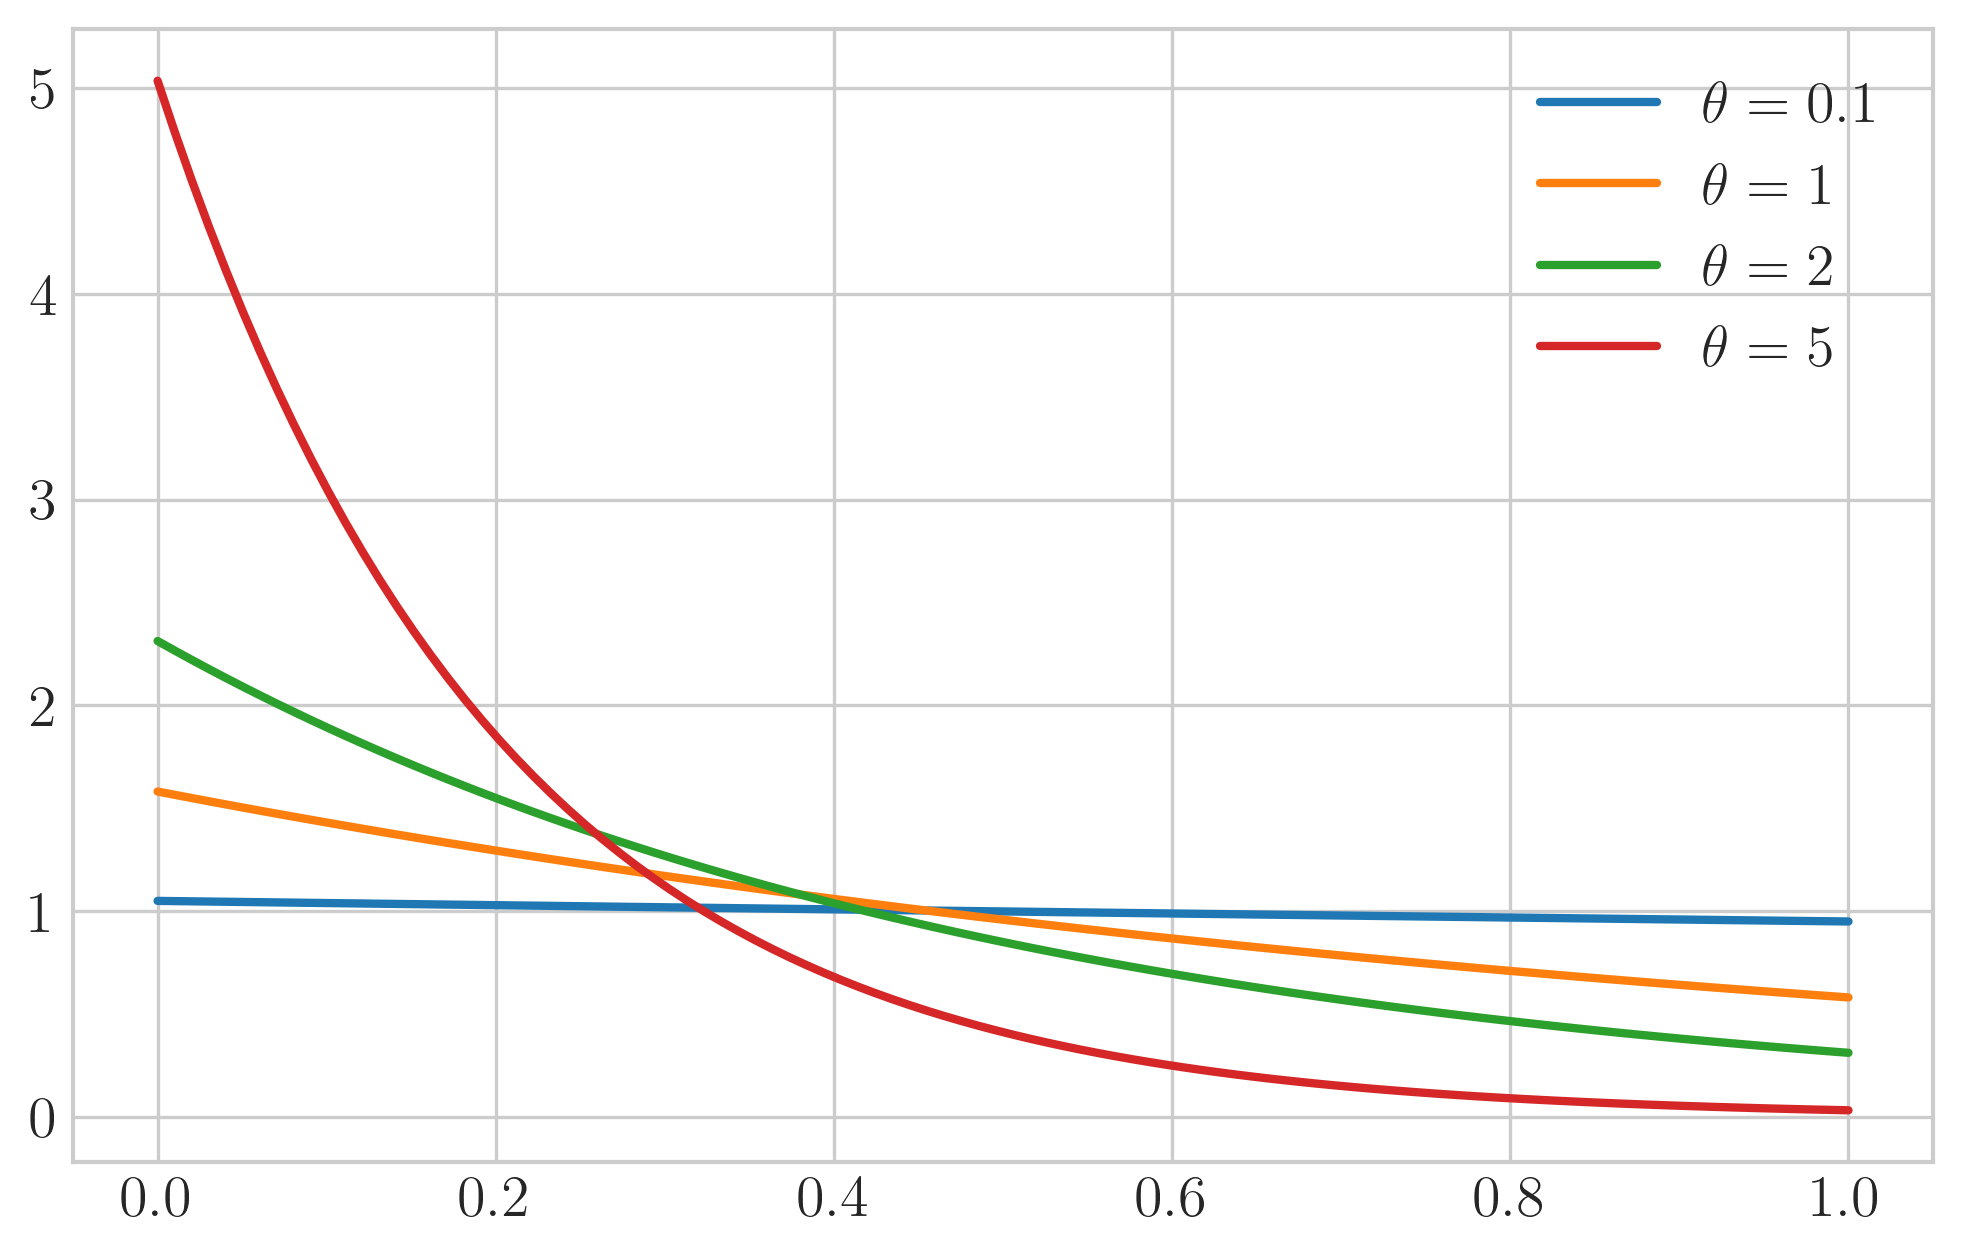
\includegraphics[scale=0.65]{plots/pdf_min_hat.png}
        \caption{Графіки щільності $f_{\widehat{m}}(x)$ для різних значень $\theta$.}
    \end{figure}
    \begin{figure}[H]
        \centering
        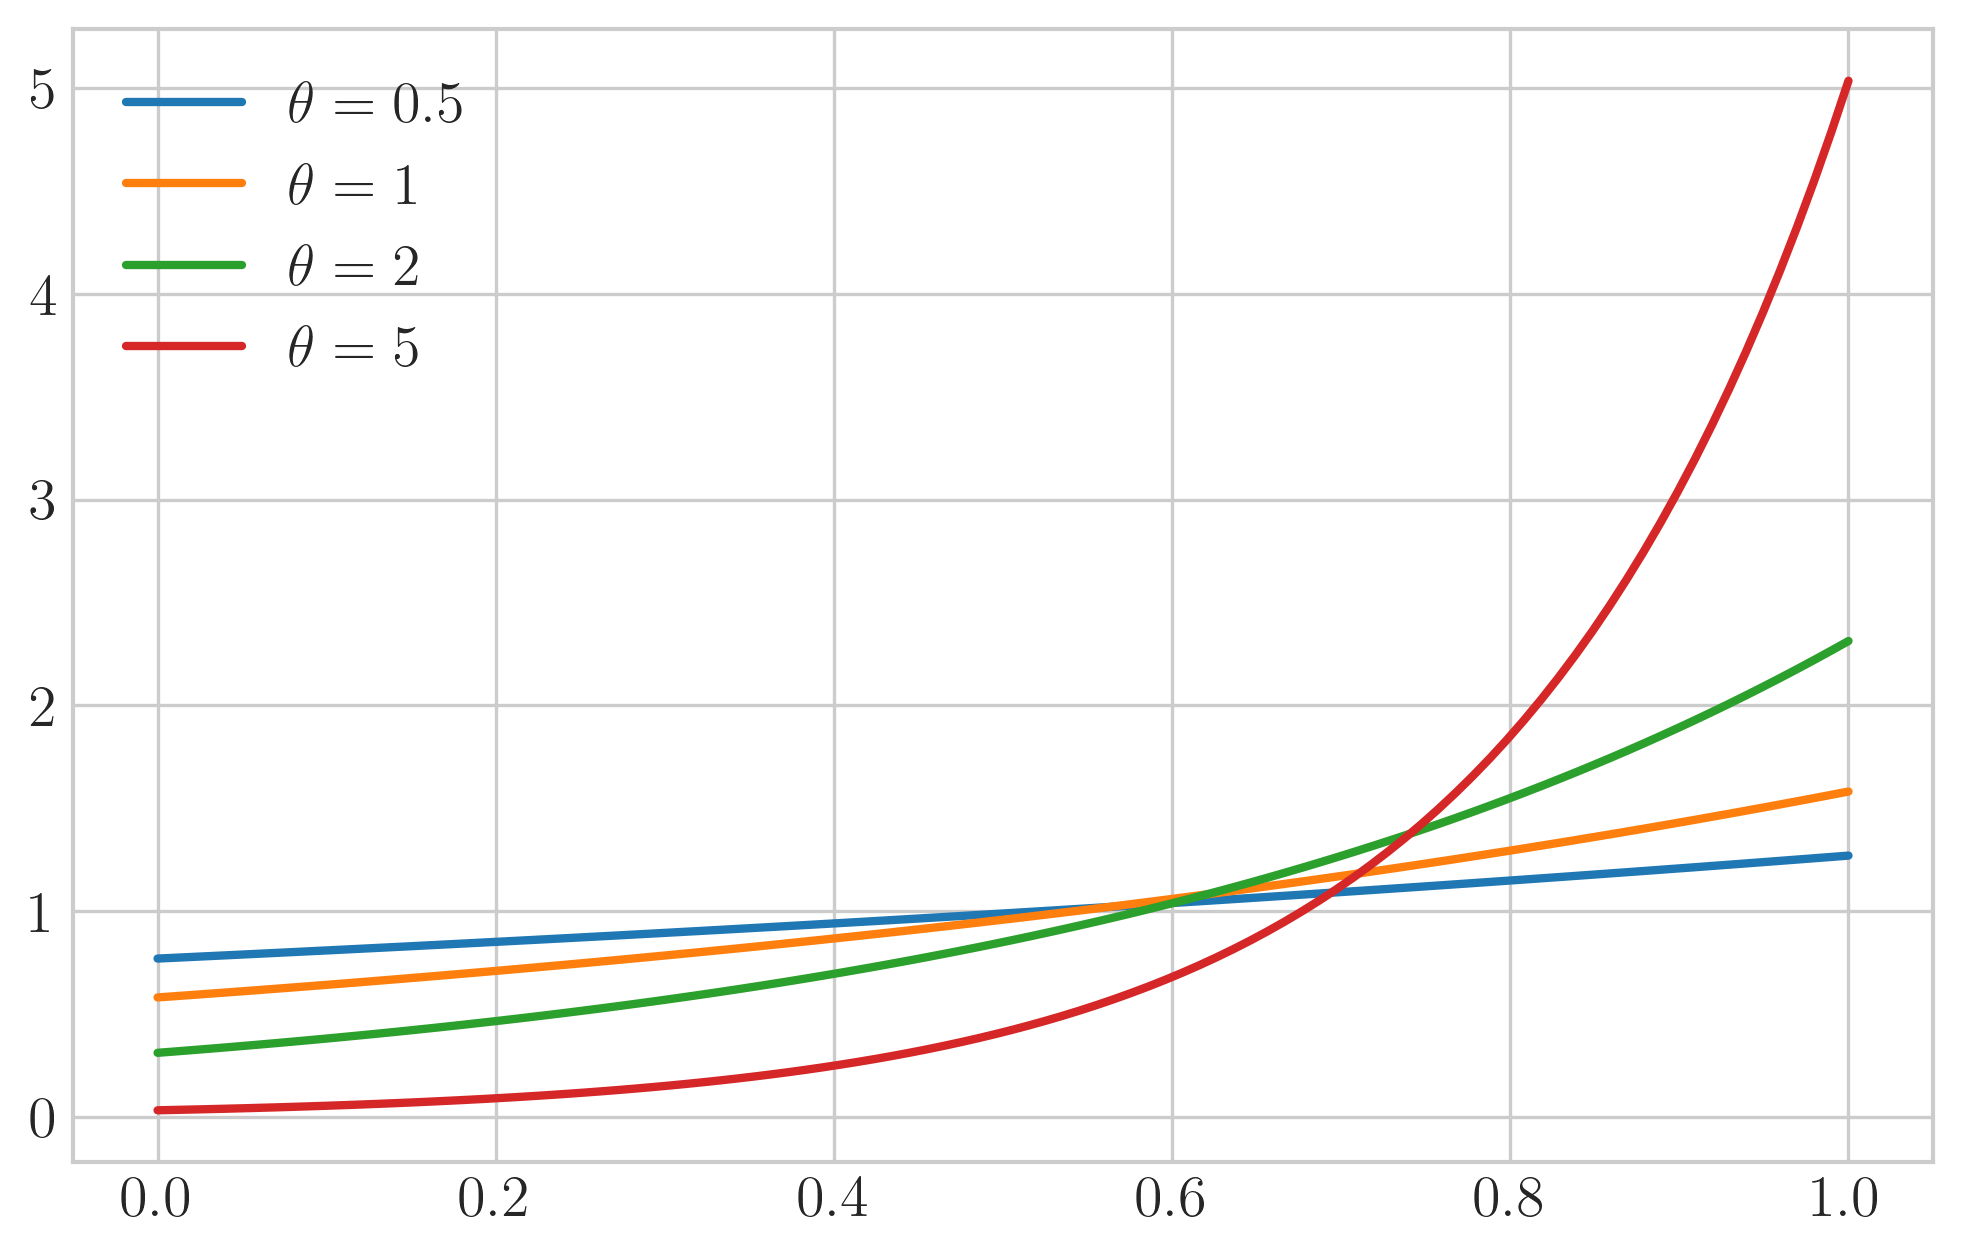
\includegraphics[scale=0.65]{plots/pdf_max_hat.png}
        \caption{Графіки щільності $f_{\widehat{M}}(x)$ для різних значень $\theta$.}
    \end{figure}
\end{theorem}